\chapter{Robust Control}

In general, a robust system is a system that is capable of meeting the requirements (which is stability or other performances) even in the presence of model uncertainties and/or disturbances. Robust control is an approach to designing a system in a way that can handle uncertainties. 

\section{Reason for a Robust control}

In general, for any system based on a mathematical model, an input / output system model is created such that, the outputs of the system measurements can be used directly / indirectly in some form by a controller. The controller then develops a control law which is then fed back into the input/output model as shown in figure \ref{fig_RobustControlReasons1}
\begin{figure}[h!]
	\centering
	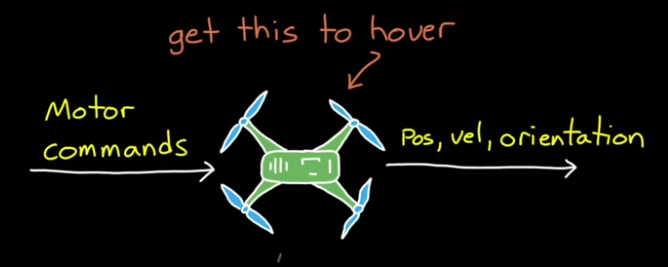
\includegraphics[width=0.6\linewidth]{Bilder/RobustControlReasons1.png}
	\caption{Input/Output model of a plant}
	\label{fig_RobustControlReasons1}
\end{figure}
In this system shown in figure \ref{fig_RobustControlReasons1}, the inputs and the outputs are labeled. Using these outputs (or measurements) from this input/output plant model, a following feedback control system can be developed as shown in \ref{fig_RobustControlReasons2}
\begin{figure}[h!]
	\centering
	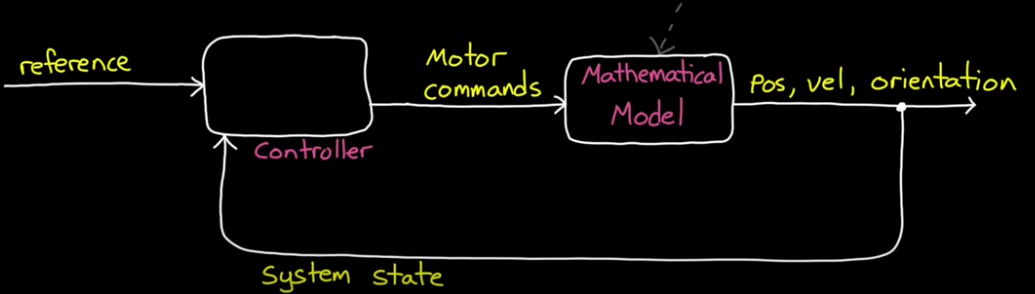
\includegraphics[width=0.6\linewidth]{Bilder/RobustControlSystemReason2.png}
	\caption{Control system developed using the measurements from the input/output model}
	\label{fig_RobustControlReasons2}
\end{figure}
the part where the controller goes could be anything from a classical designed PID to a full state feedback controllers tuned using LQR etc., as well as a neural network can be used as a control algorithm. Once the controller meets the requirements, then the control algorithm can be used to develop a C-Code and flashed into an embedded system. This controller can then be tested finally with a original system so as to verify the requirements with actual model as shown in figure \ref{fig_RobustControlReasons3}
\begin{figure}[h!]
	\centering
	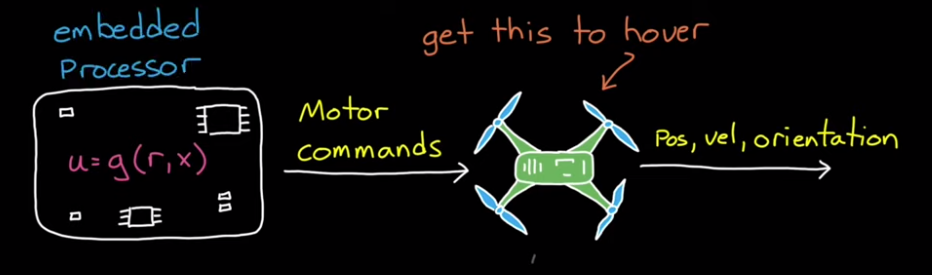
\includegraphics[width=0.6\linewidth]{Bilder/RobustControlSystem_Reasons3.png}
	\caption{Control system developed using the measurements from the input/output model}
	\label{fig_RobustControlReasons3}
\end{figure}
The validity of this controller is based on the accuracy of the model. Obviously, as the mathematical model deviates from the original model, the performance deviations also deviate accordingly or may fail entirely. This could happen in most of the real world applications as  most of the models are prone to one or more of the following reasons as to why mathematical models deviate / fail to represent the required plant model.
\begin{enumerate}
	\item \textbf{\textit{Complex Dynamics}}: It may be very complex to understand and capture complex dynamics of a system such as high frequency vibrations in a given plant system. In most of such cases, the mathematical model could not have included such complexities in order to simplify things. Even in case of black-box modeling, there would not have been relevant sensors to actually measure such complexities directly.
	\item \textbf{\textit{Uncertainties in the model}}: this could raise due to uncertain disturbances, actuator uncertainties as well as uncertainty on how the system would respond to such uncertain actautions among others.
	\item \textbf{\textit{Intentional Simplicity}}: In most of the cases, model are linearized so as to simply whole of the development process. Realism is sacrificed for simplicity. 
	\item \textbf{\textit{Stochastic events}}: this is one of the reasons where the model would naturally vary over time and th changes are driven by unknown or stochastic events. Short term of such events could be treated as noise and the long term events could be of the performance deterioration as it ages. 
	\item \textbf{\textit{Process variations}}: after producing series of products it is often noticed that there are slight variations in each of the model produced due to slight process variations which now have been taken into consideration while developing a mathematical model. 
\end{enumerate}
Due to these above mentioned model uncertainties, the controller's performance can be expected to drift as the model uncertainties begin to drift. In order to combat this model uncertainty, one of the simplest ways is to increase the band of stability. Such that the system being designed to just be stable is not enough in this case, the system is in fact designed to have some margin of stability. In such a case, as the model uncertainty pushes the stability of the system in reality, it will be only eating up this band of stability that was previously included in the design. Therefore, maintaining controller stability even in the cases of some model uncertainty variations.

The gain and phase margins discussed earlier in classical control theory does exactly this purpose. For example, if a control system is specified by a case that, gain margin > 6dB and phase margin > 45 deg. These margins say on the limits the system can deviate before  it becomes unstable. Such that, this system has 6dB of additional gain that can be added before it goes unstable, similarly, phase can be lagged upto 45 deg before the system goes unstable. Now the decision on choosing these margins depends entirely on the uncertainties. However, it should also be noted that as these margins are designed to have higher limits, it also increases the cost of the project. On the other hand, too little of these margins will also result in failed requirement testing.

It should also be noted that though gain and phase margins are very useful in determining the stability of the systems they are not a complete picture of robustness of a system. For an example consider a open-loop transfer function of  a system:
\begin{equation}
	G = \frac{0.38s^2 + 0.038 s + 0.209}{s^4 + 1.06 s^3 + 0.56 s^2 + 0.5s}
\end{equation}
the closed-loop stability can be determined by open-loop gain and phase margins, using Matlab function $margin(G)$, the following figure \ref{fig_2_ch_RC_intro_1} was generated
\begin{figure}[h!]
	\centering
	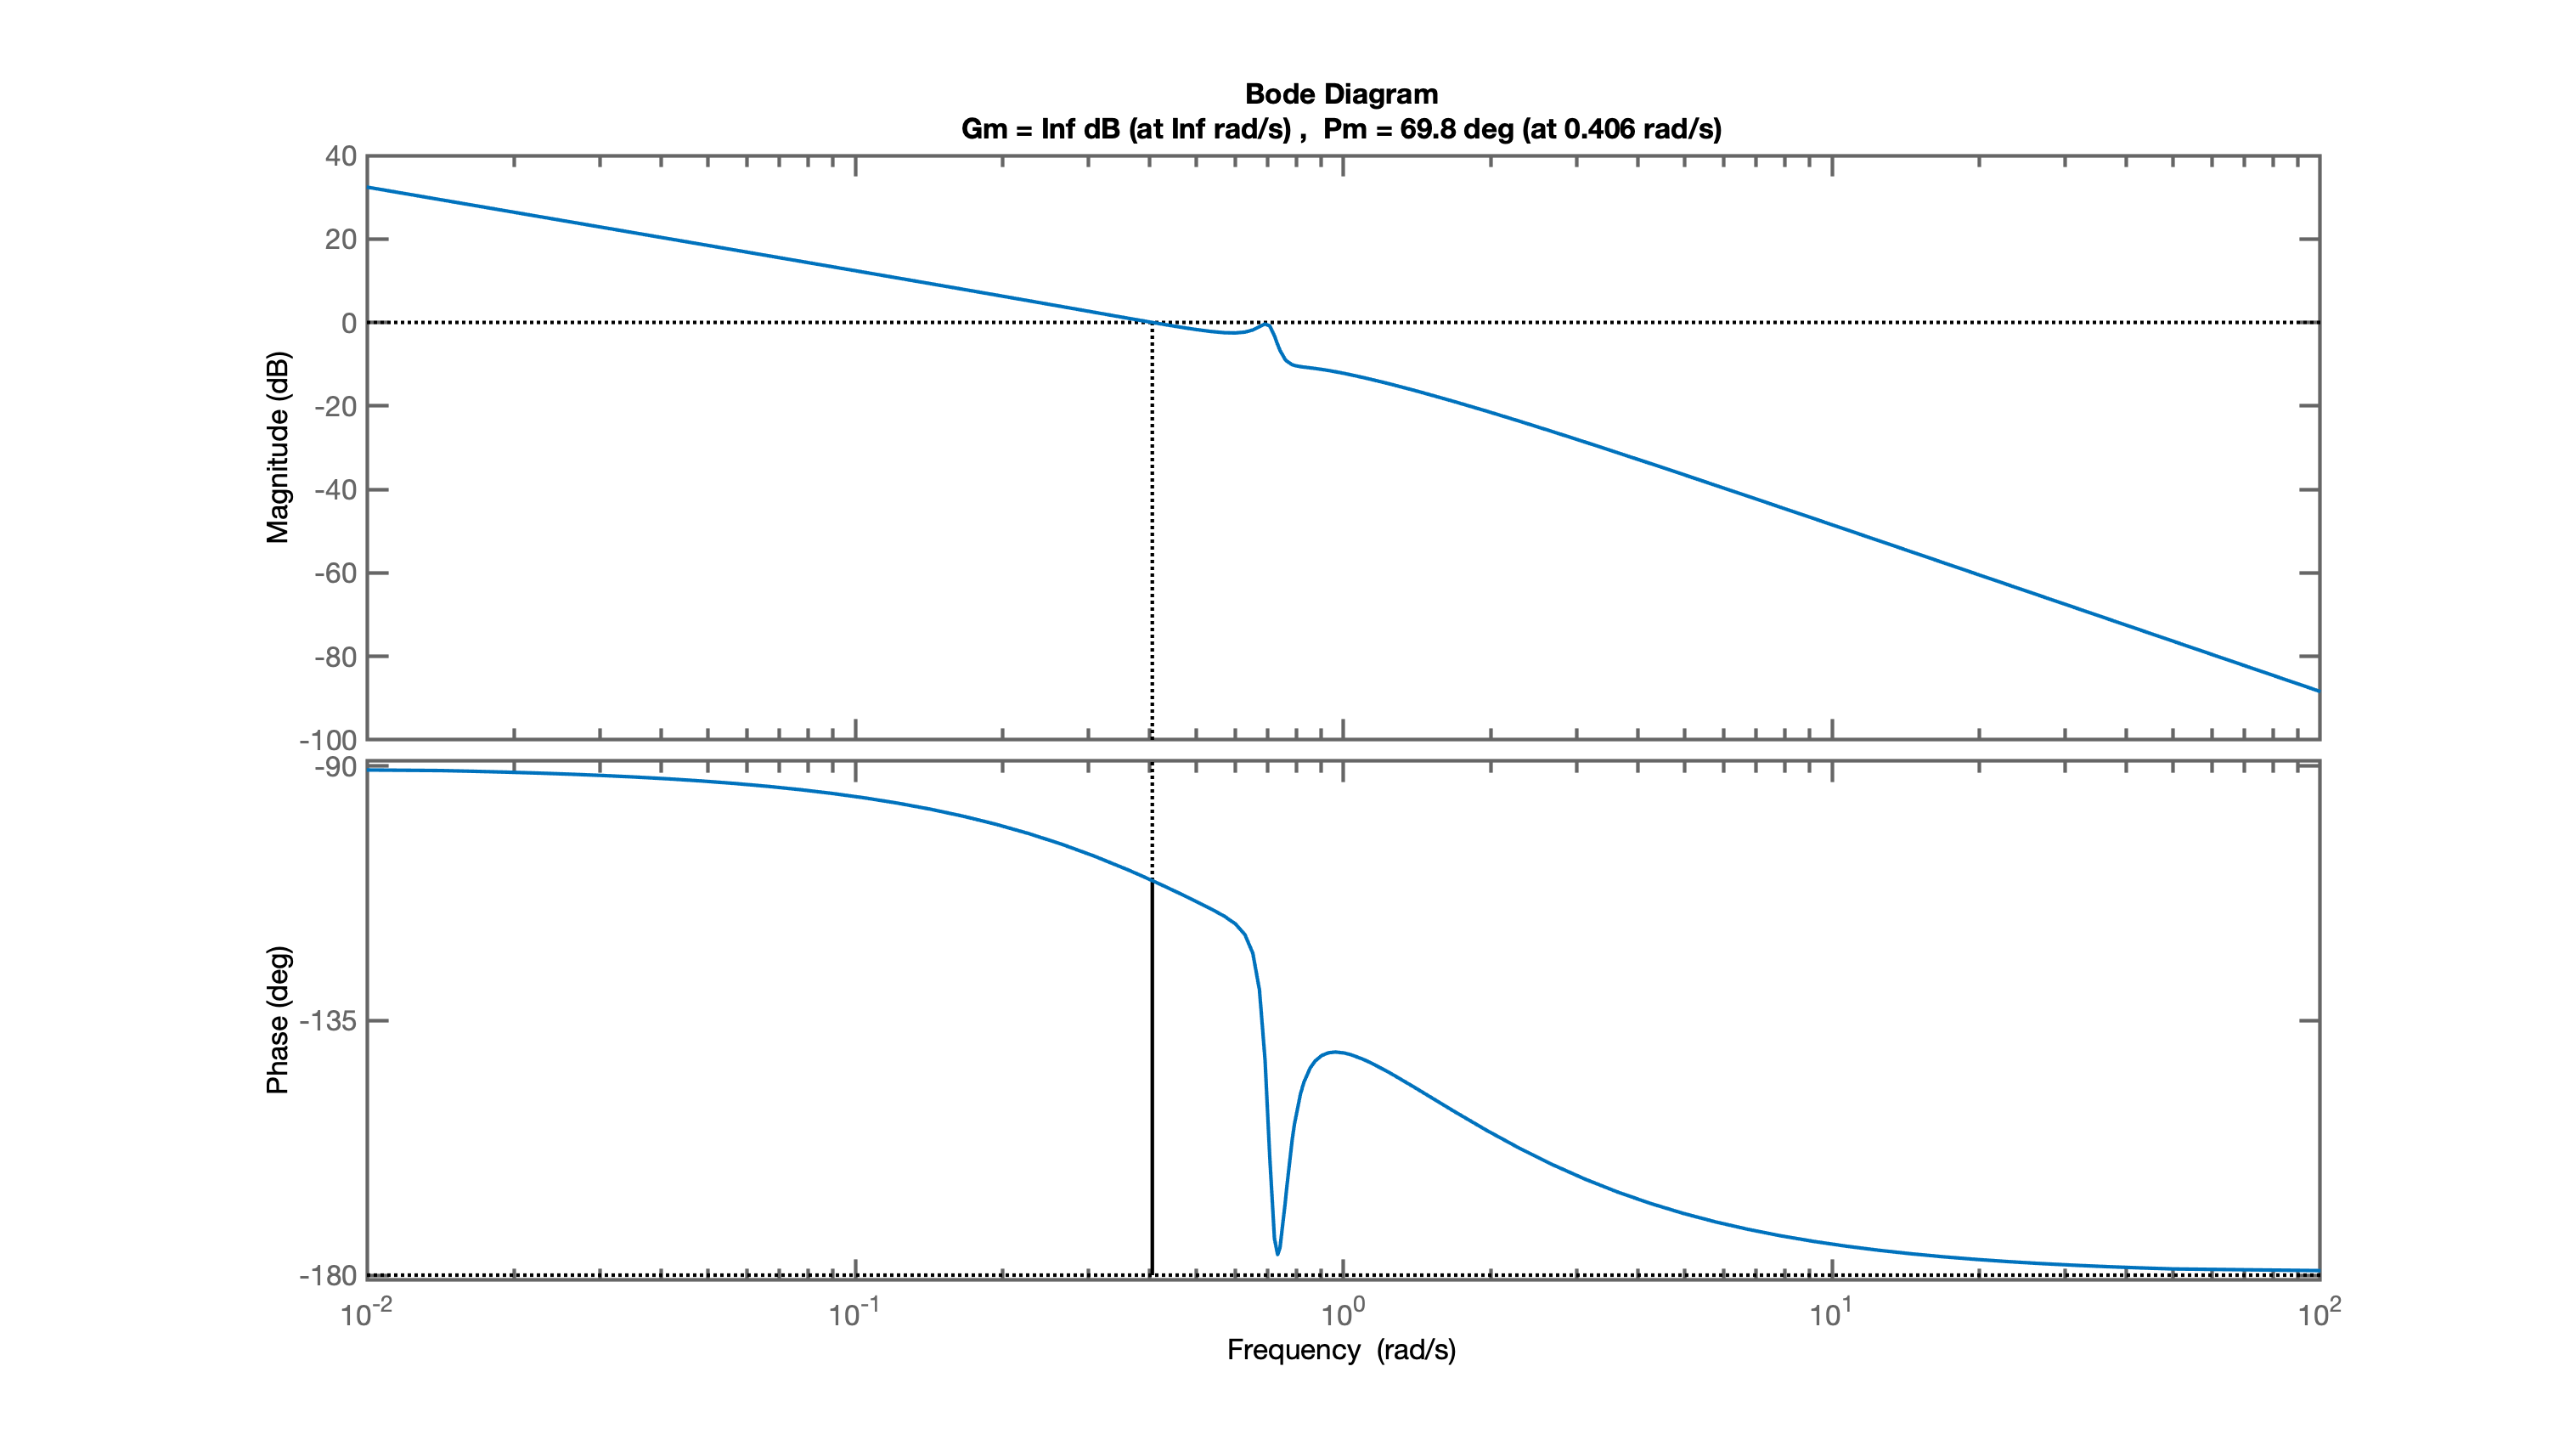
\includegraphics[width=1.2\linewidth]{Bilder/Matlab_RobustControl_Intro_1.eps}
	\caption{open-loop margins of an example system}
	\label{fig_2_ch_RC_intro_1}
\end{figure}
\newpage
It can be seen in \ref{fig_2_ch_RC_intro_1}, that the gain margin for this system is literally $\infty$, this system appears to be fairly stable under large gain additions as it can be seen in \ref{fig_2_ch_RC_intro_1}, that the phase never crosses the $180^{\circ}$ line. This can also be seen by adding a closed loop gain using Matlab's $feedback(G*addGain,1)$ which generates \ref{fig_2_ch_RC_intro_2}
\begin{figure}[h!]
	\raggedleft
	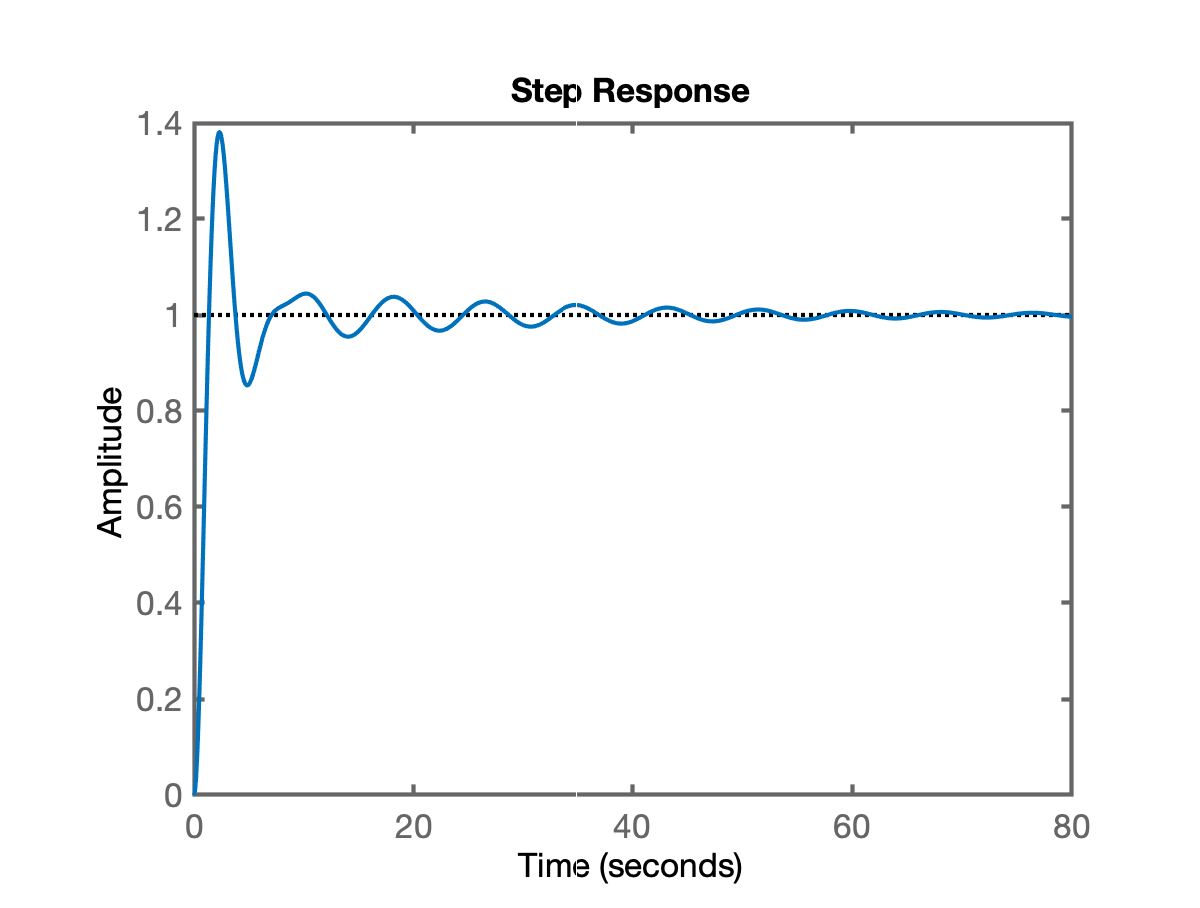
\includegraphics[width=0.75\linewidth]{Bilder/Matlab_RobustControl_Intro_2.eps}
	\caption{adding gain to the example system}
	\label{fig_2_ch_RC_intro_2}
\end{figure}
\newpage
where addGain = $10^{amplitude / 20}$ in dB and amplitude = $15$ in metric scale. further, adding phase delay of 2 sec using Matlab's $feedback(G*exp(-s*2),1)$, generates \ref{fig_2_ch_RC_intro_3}
\begin{figure}[h!]
	\centering
	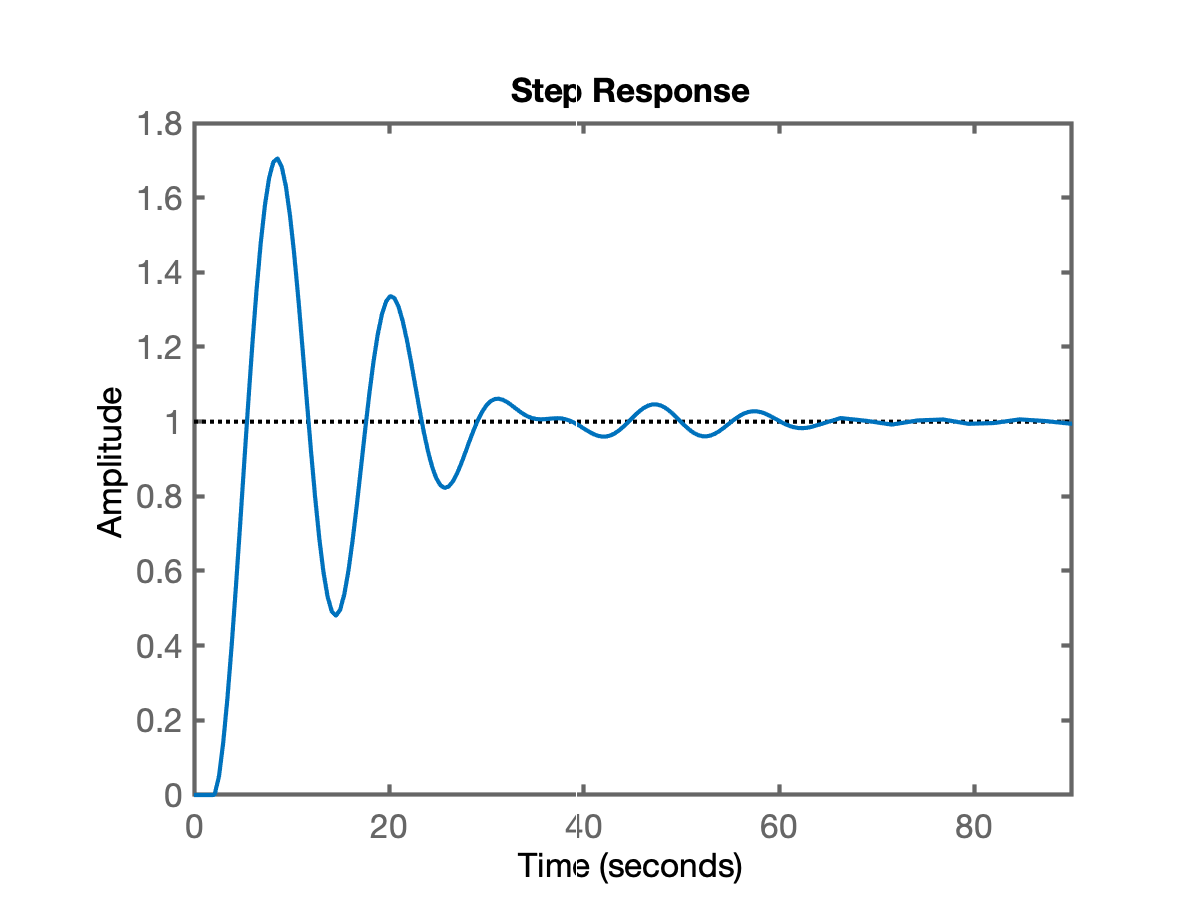
\includegraphics[width=0.75\linewidth]{Bilder/Matlab_RobustControl_Intro_3.eps}
	\caption{adding phase to the example system}
	\label{fig_2_ch_RC_intro_3}
\end{figure}
\newpage
But when the system is added with both gain and phase margins, the system would go completely unstable as shown in \ref{fig_2_ch_RC_intro_4}
\begin{figure}[h!]
	\centering
	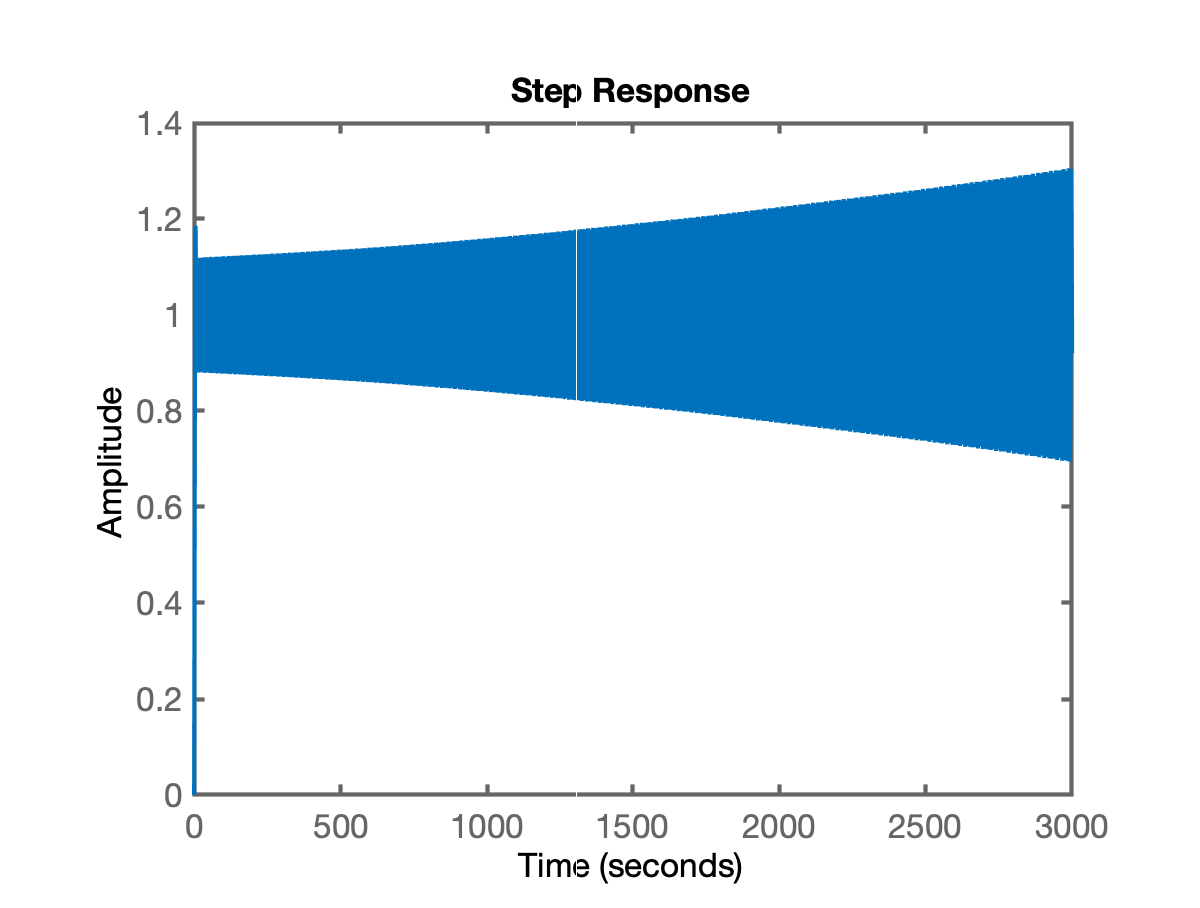
\includegraphics[width=0.75\linewidth]{Bilder/Matlab_RobustControl_Intro_4.eps}
	\caption{adding phase to the example system}
	\label{fig_2_ch_RC_intro_4}
\end{figure}
this is due to the combined effect of adding both the margins together which cannot be determined only using the bode plots. Therefore, in robust control theory, another concept called disk margin is used which accounts for both gain and phase margins simultaneously. Disk margins further also have an advantage of being able to be implemented to MIMO systems which unlike in classical margins (from bode plot) is not in general easy to be implemented. By using Matlab's $diskmargin(G)$, the following structure is generated
\begin{lstlisting}
	struct with fields:
	
		GainMargin: [0.7379 1.3552]
		PhaseMargin: [-17.1526 17.1526]
		DiskMargin: 0.3016
		LowerBound: 0.3016
		UpperBound: 0.3016
		Frequency: 0.7137
\end{lstlisting}
from this struct it can be seen that the actual gain and phase margins are actually $1.3552$ and $17.1526$ which is much lower than what was originally determined using classical gain and phase margins. Now, lets plot a step repsonse again using these new results generated using disk margins,
\begin{figure}[h!]
	\centering
	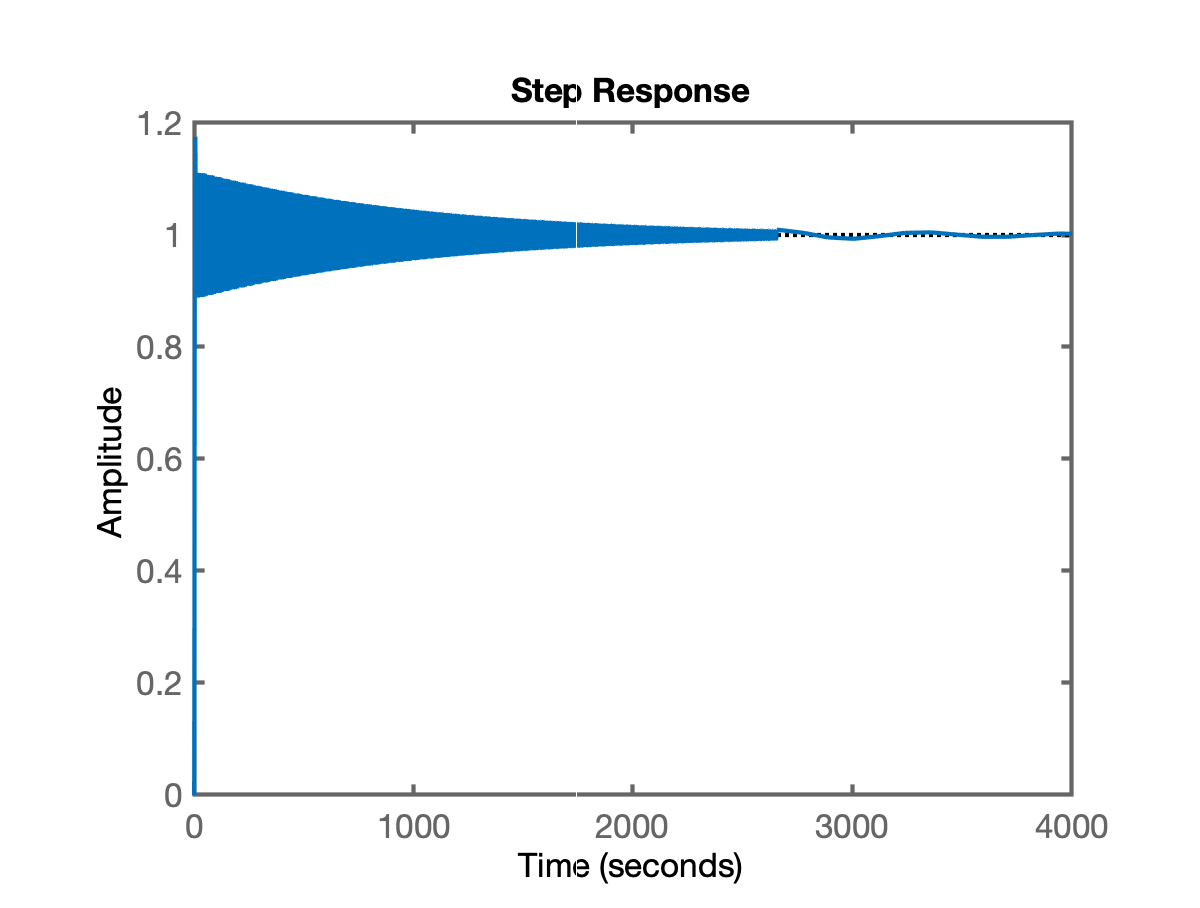
\includegraphics[width=0.75\linewidth]{Bilder/Matlab_RobustControl_Intro_5.eps}
	\caption{adding phase to the example system}
	\label{fig_2_ch_RC_intro_5}
\end{figure}
\newpage
To summarize this intrduction, for robust control analysis, it is important to asses and scale the model variations and other disturbances into the system before desigining the controller. In most of the cases, it is not possbile to know in prior how exactly the model would vary and how other parameters such as sensor noise or high frequency dynamics would make the model uncertain. However, it is possbile to predict how these uncertainities would possible develop during real time operations of the system. These uncertainties can be modeled as some schotiastic disturbution of disturbances that goes into the system and therefore, a valid range of band limits can be implemented directly into the system while designing the system. Other than schotiastic modeling there are other simple ways to model there uncertainities such as in case of classical modeling approach, one can conside that only the gain margin or only the phase margin to designed with. In some of the real time systems for example, one can have more certainty of system perforamce at lower operating frequencies that at higher opearting frequencies. In such cases, a lower band limit at lower frequencies and higher band limit at higher operating frequencies can be implemented into the design.

So far in this introduction only the analysis part of robust control methdology has been discussed. For the sythesis part (deisgn the controller), it should be noted that in case of a robust controller, it is not the case that there is a specific controller such as a PID or a full state feedbak controller. Rather, a robust control discusses a methodology to tune controller parameters such as PID to make the system robust. 

In classical control syntesis, in book a breif introduction is already provided earlier for a robust control design usign loop shaping (root locus and Bode plots) by adding poles or zeros, to make the system more robust in case of uncertatinities. However, this classical method is not suitable for MIMO system and we have other methods such as $H_{\infty}$ or $\mu$ synthesis.

In all cases, it is important to note that the basis of robust control analysis and synthesis is pure basd on adressing uncertainities.  For this the following points have to be noted
\begin{enumerate}
	\item understand uncertainities and represent them in the model
	\item analyse the system to see if the system is still stable with these added uncertainities
	\item if not, then tweak the design based in robust controll analysis and synthesis such that the system is stable again
\end{enumerate}
